\section{Application, implications, and limitations}
\label{sec:case}

\subsection{Application and what-if analysis}

We instantiate Problem~\ref{prob:sizing} on $\approx3\times10^{7}$ ballots over
twelve hours ($\Dpk\approx2.1\times10^{3}$~TPS), requiring detection of a
coordinated omission fault of fraction $\phi=0.2$ within one epoch at level
$1-\epss$. Absolute demand enters via scale-up $\kappaScale$ from \RNM{} units.
With free $\kappaScale$, Problem~\ref{prob:sizing} takes
\begin{equation}
\kappaScale^{\star}
=\frac{\Dpk}{\underline{\TPSn}_{1-\epsp}(4,\cc^{\star})},
\label{eq:kappa}
\end{equation}
the minimal scale at which the lower PI bound at $\n=4$ meets $\Dpk$.

\paragraph{Scenario A (baseline).}
Substituting the calibrated coefficients
($\beta=\resBeta$, $\gamma=\resGamma$) at $\cc^{\star}=\resCstar$ yields
$\kappaScale=\resKappa$ and feasibility window
$[\resNminCase,\resNmaxCase]$ with $\nopt=\resNoptCase$
(Proposition~\ref{prop:window}; Figure~\ref{fig:window}). Under this demand and
hardware class the window collapses to a single admissible count: the network is
throughput-bound at the smallest BFT set admitted by the formulation.

\begin{figure}[!t]
\centering
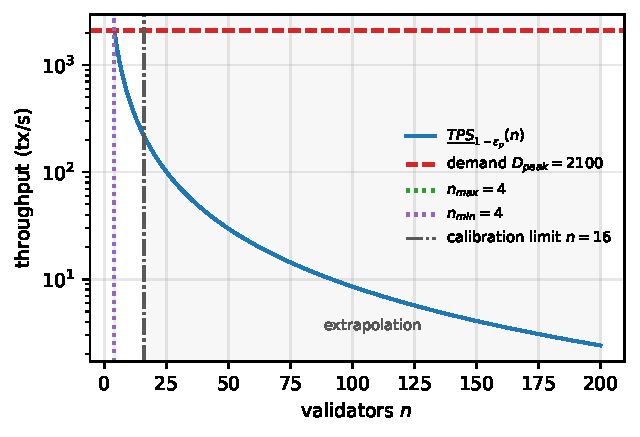
\includegraphics[width=0.42\textwidth]{figures/fig_window}
\caption{Scenario~A: at minimal admissible $\kappaScale=\resKappa$, the
feasibility window is $[\nmin,\nmax]=[\resNminCase,\resNmaxCase]$. The
dash-dotted line marks the calibration limit $\n=\resNmaxMeasured$; the shaded
region to its right is model-based extrapolation}
\label{fig:window}
\end{figure}

\paragraph{Scenario B (doubled peak demand, fixed hardware class).}
Hold $\kappaScale=\resKappa$ and replace $\Dpk$ by $2\Dpk$. Then $h$
in~\eqref{eq:h} falls by $\log 2$ everywhere; in particular $h(4)<0$, so the
feasible set is empty (Corollary~\ref{cor:infeasible}). Within the calibrated
law, doubling peak load on the same hardware class is an architectural
impossibility: adding validators cannot restore feasibility, because throughput
falls with~$\n$.

\paragraph{Scenario C (WAN deployment, fixed hardware class).}
Retain $\kappaScale=\resKappa$ and $\Dpk$, but substitute the high-RTT
exponent $\beta=\resBetaRttHigh$ (X4) for $\beta=\resBetaRttZero$. The steeper
penalty yields $h(4)<0$ and an empty window: a hardware class that is
marginally admissible under LAN $\beta$ becomes infeasible under WAN $\beta$
without raising $\kappaScale$.

The workflow applies equally to registry and identity sizing under analogous
demand assumptions; binding elections on a blockchain remain outside the
recommendation \cite{springall2014,specter2020,park2021}.

\subsection{What this implies}
\label{sec:discussion}

A fitted $(\beta,\gamma)$ transfers when concurrency path, quota regime, and
RTT class match the calibration. Our results suggest that future benchmarks
should report $\lambda$ (or $\lambda=0$), per-validator quota, and RTT class
(Corollary~\ref{cor:sign}).

\subsection{Limitations}
\label{sec:limitations}

\emph{Fault class.} Encrypted transport limits X5 to omission/duplication
(AUC~$\resAuc$; throughput-bound window).

\emph{Infrastructure and range.} Experiments use commodity four-core CI with
$\n\le\resNmaxMeasured$. Beyond that range, extrapolation is model-based and
is quantified by prediction intervals.

\emph{Coefficients versus methodology.} Numerical $(\beta,\gamma)$ are
Besu/QBFT-specific. Proposition~\ref{prop:identifiability} is analytical under
model assumptions; the campaign shows consistency within the investigated
configuration. The \RNM{} protocol and chance-constrained workflow are intended
to generalize under matching measurement conditions; production scale-up uses
$\kappaScale$ in~\eqref{eq:kappa}.

